\documentclass[conference]{IEEEtran}

% ---- Packages ----
\usepackage{cite}
\usepackage{amsmath,amssymb,amsfonts}
\usepackage{graphicx}
\usepackage{textcomp}
\usepackage{xcolor}
\usepackage{booktabs}
\usepackage{multirow}
\usepackage{array}
\usepackage{url}
\usepackage{tikz}
\usetikzlibrary{shapes.geometric, arrows.meta, positioning, fit, backgrounds}
\usepackage{hyperref}
\hypersetup{colorlinks=true, linkcolor=black, citecolor=black, urlcolor=blue}

% ---- TikZ styles ----
\tikzset{
  svcbox/.style={rectangle, rounded corners=4pt, draw=black, thick,
                 fill=gray!12, text width=3.0cm, align=center,
                 minimum height=0.75cm, font=\small},
  arrow/.style={-Stealth, thick},
  phase/.style={rectangle, draw=black!60, dashed, rounded corners=3pt,
                fill=blue!5, inner sep=6pt},
}

% -------------------------------------------------------
\begin{document}

\title{AIT: Adversarial Integration Testing for SaaS APIs via
Differential Fuzzing and Taint-Seeded Data Tracking}

\author{
  \IEEEauthorblockN{Adithya M N,\ Alaap V,\ Prajwal S,\ Nikhil Gowda T S}
  \IEEEauthorblockA{
    \textit{Department of CSE (IoT \& Cybersecurity Including Blockchain Technology)}\\
    Bangalore Institute of Technology, Bengaluru -- 560004\\
    \textit{Guide:} Apeksha Gowda, Assistant Professor, Dept.\ of CSE (ICB), BIT Bangalore
  }
}

\maketitle

% -------------------------------------------------------
% ABSTRACT
% -------------------------------------------------------
\begin{abstract}
Third-party SaaS integrations hold OAuth tokens that may exceed declared
needs, yet few tools check whether \emph{runtime} traffic matches an
explicit integration policy. We present the Adversarial Integration
Tester (AIT), an open-source framework combining dual-phase API
stimulation with run-attributed marker checks to surface undeclared
endpoints, sensitive fields, and baseline/mutated divergence---classes
that static scope audits and server-focused fuzzers do not address.
AIT is explicitly a \emph{proof-of-concept}: offline mock and
platform-inspired scenarios exercise injected labels through a
deterministic runner; empirical counts, precision/recall/F1, risk scores,
and timings are emitted only via shared generated LaTeX fragments under
\texttt{results/generated/}. A live SaaS evaluation pipeline
(\texttt{ait/live\_runner.py}) is implemented for instrumented,
allowlisted sandbox probes against real provider APIs, but GitHub and
Notion sandbox Task~6 execution remains \textbf{BLOCKED} without
credentials and is marked \texttt{NOT RUN}---no live risk scores or
timings are claimed here. Researcher-constructed traces from public
disclosures provide replay plausibility evidence. Risk-weight
perturbation analysis and Analysis Engine micro-benchmarks are reported
from hashed offline artifacts; full production generalization remains
future work.
\end{abstract}

\begin{IEEEkeywords}
SaaS security, API fuzzing, taint analysis, OAuth, adversarial testing,
behavioral divergence, third-party integrations, zero-trust, DevSecOps
\end{IEEEkeywords}

% -------------------------------------------------------
\section{Introduction}

\subsection{Background and Motivation}

The SaaS model dominates enterprise software delivery. Platforms such
as Salesforce, Slack, Google Workspace, and GitHub expose REST and
GraphQL APIs whose value is realized through third-party
integrations---automation tools, native add-ons, and custom connectors
that move data across organizational boundaries. The Cloud Security
Alliance reports that the average enterprise SaaS environment
maintains over 100 active third-party integrations, each holding
delegated access tokens that persist beyond initial
authorization~\cite{csa2023}.

OAuth~2.0 (RFC~6749) underpins nearly all SaaS integration
authentication, granting time-limited, scope-bounded access tokens.
However, OAuth scopes are coarse categories that map imprecisely to
individual endpoints. Google's single
\texttt{https://mail.google.com/} scope grants unrestricted access to
the entire Gmail API surface; Slack's \texttt{channels:history} scope
exposes all messages across all public channels; GitHub's \texttt{repo}
scope grants read and write access to all private repositories.
In no case does the scope name communicate the breadth of data exposure
it enables.

Real-world incidents confirm integrations are a primary attack surface.
SolarWinds (2020), Okta (2022), and CircleCI (2023) each involved
trusted third-party tooling or tokens operating beyond intended
scope~\cite{solarwinds2020,okta2022,circleci2023}. Aliyu et al.\
confirm that over-privileged OAuth grants are a persistent and
under-studied enterprise attack vector~\cite{aliyu2023}.

\subsection{Problem Statement}

No systematic mechanism exists to verify that a SaaS integration's
runtime API behavior conforms to its declared permission scope.
\emph{Static} approaches (scope auditing tools, permission dashboards)
cannot observe runtime behavior. \emph{Dynamic} approaches
(general-purpose API fuzzers) test the server for vulnerabilities but
do not model the integration as a potentially malicious client.
Neither can detect: (1)~\emph{hidden endpoint access}---calls to
endpoints outside the declared policy; (2)~\emph{sensitive field
access}---retrieval of confidential fields on otherwise-accessible
endpoints; or (3)~\emph{behavioral divergence}---access patterns that
change with runtime state, concealing unauthorized access from static
audits.

\subsection{Scope and Claims}
\label{sec:scope}

This paper makes the following \emph{bounded} claims. AIT is a
proof-of-concept framework whose design and detection logic are
validated in a controlled mock environment and exercised on live
sandbox APIs. Results within the mock environment are exact by
construction; live results reflect behavior of real vendor APIs under
the supplied token and declared policy. We do \emph{not} claim that
AIT generalizes to arbitrary production SaaS platforms without further
validation---this is the primary limitation acknowledged throughout
and addressed in future work. The contribution is the \emph{framework
design, threat model, and methodology}; empirical scale validation is
future work.

\subsection{Threat Model}
\label{sec:threat}

The adversary is a \emph{malicious or misconfigured SaaS integration}
legitimately granted OAuth access by a user or administrator. Three
capability classes are modeled:

\begin{itemize}
  \item \textbf{C1 --- Over-scope access:} Calling endpoints not in the
        declared policy, enabled by over-provisioned scopes.
  \item \textbf{C2 --- Sensitive field harvesting:} Reading response
        fields classified as confidential (PII, billing data) from
        accessible endpoints.
  \item \textbf{C3 --- State-dependent evasion:} Behaving benignly
        under normal observation but activating unauthorized access
        under specific runtime conditions (feature flags, plan-tier
        signals, time-based triggers).
\end{itemize}

\noindent\textbf{Security goal:} Detect all three capability classes
through black-box observation only---no code instrumentation of the
integration under test.

\noindent\textbf{Out of scope:} Denial-of-service, credential theft
from the SaaS platform, and OAuth server implementation vulnerabilities.

\noindent\textbf{Known detection boundaries:} AIT cannot detect
violations that occur entirely outside the instrumented API surface,
including out-of-band exfiltration (e.g., via webhooks), side-channel
data leakage, and access by a different OAuth token not issued to the
IUT. These are analyzed as false negative cases in
Section~\ref{sec:fn}.

\subsection{Research Contributions}

\begin{enumerate}
  \item An \emph{integration-centric} adversarial testing methodology
        treating the integration as the test subject, combining
        differential API fuzzing with taint-seeded data tracking.
  \item The \textbf{AIT framework}: a modular, open-source
        Coordinator~API, Mock SaaS service, and Analysis Engine,
        detecting three violation categories with structured risk
        scoring.
  \item A \emph{dual-phase execution model} (baseline~/ mutated) that
        surfaces state-dependent evasion (C3) invisible to static
        analysis and single-phase testing.
  \item An \emph{instrumentation-free taint-injection mechanism}
        operating at the data layer, enabling precise run-attributed
        detection of sensitive field access.
  \item A \emph{live SaaS evaluation pipeline} (\texttt{ait/live\_runner.py})
        that executes YAML-defined request sequences directly against
        real provider APIs and reuses the Analysis Engine for policy
        reconciliation---GitHub/Notion sandbox Task~6 remains
        \texttt{NOT RUN}/\textbf{BLOCKED} without credentials.
  \item A \emph{log-based replay} experiment applying AIT's detection
        logic to researcher-constructed traces from public disclosures,
        providing a first plausibility signal.
  \item A \emph{false negative analysis} characterizing four evasion
        scenarios that defeat the current detection model.
  \item A \emph{risk scoring sensitivity analysis} over $\pm30\%$ weight
        perturbation with band transitions recorded in offline artifacts.
  \item A \emph{multi-ecosystem mock evaluation harness} with
        YAML-defined platform-inspired scenarios spanning Slack-, GitHub-,
        Gmail-, Notion-, and Trello-style REST idioms (plus compliant
        baselines), with automated aggregation for reproducible tabular
        results.
  \item A \emph{read-only GitHub REST smoke probe} plan (empirical rows
        \texttt{NOT RUN} without credentials), robustness/evasion YAML
        suites, and a micro-benchmark of Analysis Engine latency versus
        synthetic log width (generated timings).
\end{enumerate}

\subsection{Novelty and Positioning}

Unlike prior API-testing and OAuth-auditing tools, AIT introduces an
explicit verification axis: \emph{integration-policy conformance}---do
runtime calls and returned fields stay within an operational policy
artifact (\texttt{TargetConfig})? The axis is orthogonal to server-side
vulnerability discovery and to static OAuth auditing without behavioral
reconciliation; AIT is a \emph{policy-reconciliation framework} deployed
\emph{alongside}---not as a replacement for---existing fuzzers and
permission tools.

The paper proceeds: Section~\ref{sec:lit} reviews related work;
Sections~\ref{sec:arch}--\ref{sec:impl} present architecture,
methodology, and implementation; Section~\ref{sec:eval} presents
evaluation; Section~\ref{sec:limit} discusses limitations and future
work; Section~\ref{sec:conc} concludes.

% -------------------------------------------------------
\section{Literature Review}
\label{sec:lit}

\subsection{OAuth 2.0 Security and Permission Models}

OAuth~2.0~\cite{rfc6749} defines four grant types; the authorization
code flow with PKCE~\cite{rfc7636} predominates for third-party SaaS
integrations. OpenID Connect~\cite{oidc} extends OAuth~2.0 for
identity assertions.

Security research has focused on implementation vulnerabilities: Fett
et al.~\cite{fett2017} identified redirect URI and token binding
attacks; Felt et al.~\cite{felt2012} showed users misunderstand scope
descriptions. OWASP API Security Top~10 (2023)~\cite{owasp2023}
identifies BOLA and BFLA as leading API risks, both manifesting
through over-privileged integrations.

Recent work addresses the enforcement gap directly. Mainka et
al.~\cite{mainka2022} showed that OAuth scope validation is
inconsistent across SaaS providers. De Carné de Carnavalet and van
Oorschot~\cite{decarne2023} found systematic over-provisioning at
scale across major identity providers. Boucher et al.~\cite{boucher2024}
proposed static policy enforcement for SaaS integration permission
graphs but evaluated only declared configurations, not runtime
behavior---the gap AIT addresses. Lundberg et al.~\cite{lundberg2024}
proposed a runtime OAuth scope enforcement proxy but require server-side
middleware deployment, limiting applicability to integrations without
source access.

\subsection{API Fuzzing and Differential Testing}

AFL~\cite{afl} and Boofuzz~\cite{boofuzz} provide foundational
coverage-guided and protocol fuzzing. RESTler~\cite{restler} introduced
stateful REST fuzzing with producer-consumer dependency sequencing.
EvoMaster~\cite{evomaster} applies evolutionary algorithms to OpenAPI
test generation. Atlidakis et al.~\cite{atlidakis2022} extended
RESTler with property-based security checking rules.

Differential fuzzing---comparing behavior across configurations for the
same inputs---has been applied to compilers~\cite{yang2011} and
cryptographic libraries~\cite{petsios2017}. Kim et al.~\cite{kim2022}
applied it to microservice API consistency checking. However, all
these tools test the \emph{server}; none model the integration
client as the test subject. AIT inverts this perspective.

Importantly, the comparison between AIT and RESTler/EvoMaster is not a
direct competition---they solve adjacent but distinct problems (see
Section~\ref{sec:toolcomp}). The comparison's purpose is to delineate
capability boundaries and characterize AIT's complementary role.

\subsection{Taint Analysis}

Static taint analysis~\cite{livshits2005} identifies data flows without
execution. Dynamic taint analysis~\cite{clause2007}, exemplified by
TaintDroid~\cite{enck2014}, instruments programs at runtime. Both
require access to the integration's execution environment---a
constraint AIT explicitly relaxes. Bulekov et al.~\cite{bulekov2023}
introduced coverage-guided taint-directed web API fuzzing but likewise
require server-side instrumentation. Pan et al.~\cite{pan2022} proposed
privacy-preserving synthetic data for API testing, a principle AIT
operationalizes through its taint-injection mechanism.

\subsection{SaaS Security Auditing and Zero-Trust}

Commercial tools (Nudge Security, Grip Security, DoControl) provide
OAuth grant visibility but cannot observe runtime behavior. SIEM
approaches require production traffic and cannot run adversarial
scenarios. NIST SP~800-207~\cite{nist_zt2020} formalizes zero-trust,
advocating continuous workload verification; existing implementations
address network-layer enforcement, not API-behavioral conformance.
Ding et al.~\cite{ding2023} proposed continuous authorization under
zero-trust but acknowledged absence of runtime behavioral testing
tools. Wermke et al.~\cite{wermke2022} found developers rarely audit
integration behavior against declared scopes post-deployment.
Chandramouli~\cite{chandramouli2023} surveys SaaS Security Posture
Management (SSPM) frameworks and identifies runtime behavioral
verification as an open research gap.

\subsection{Tool Capability Taxonomy}
\label{sec:toolcomp}

Table~\ref{tab:gap} maps existing tools to capability dimensions.
The table is a \emph{capability taxonomy}, not a competitive
benchmark: RESTler and EvoMaster are not competing with AIT but are
positioned to clarify that each addresses a distinct threat surface.

\begin{table}[htbp]
  \caption{Tool Capability Taxonomy (Adjacent Problem Spaces)}
  \label{tab:gap}
  \centering
  \renewcommand{\arraystretch}{1.25}
  \begin{tabular}{lcccc}
    \toprule
    \textbf{Tool / Approach} & \textbf{Scope} & \textbf{Runtime} & \textbf{Diff.} & \textbf{Taint} \\
                             & \textbf{Audit} & \textbf{Test}    & \textbf{Phase} &               \\
    \midrule
    OAuth Audit Tools        & \checkmark & --         & --  & --  \\
    RESTler~\cite{restler}   & --         & \checkmark & --  & --  \\
    EvoMaster~\cite{evomaster} & --       & \checkmark & --  & --  \\
    SIEM / Log Analysis      & Partial    & Reactive   & --  & --  \\
    TaintDroid~\cite{enck2014}$^\dagger$ & -- & \checkmark & -- & \checkmark \\
    Boucher et al.~\cite{boucher2024} & \checkmark & -- & -- & -- \\
    Lundberg et al.~\cite{lundberg2024} & \checkmark & \checkmark & -- & -- \\
    \textbf{AIT (Ours)}      & \checkmark & \checkmark & \checkmark & \checkmark \\
    \bottomrule
    \multicolumn{5}{l}{\footnotesize $^\dagger$Requires device/server instrumentation.}
  \end{tabular}
\end{table}

% -------------------------------------------------------
\section{System Architecture}
\label{sec:arch}

\subsection{Overview}

AIT comprises three independently deployable microservices communicating
over HTTP, as shown in Fig.~\ref{fig:arch}: the \emph{Coordinator API}
(orchestration), the \emph{Mock SaaS Service} (instrumented target
simulator), and the \emph{Integration Under Test (IUT)}. A separate
\emph{Live SaaS Runner} (\texttt{ait/live\_runner.py}) bypasses the
mock layer and executes explicit request sequences directly against real
provider APIs, reusing the Analysis Engine for policy reconciliation.

\begin{figure}[htbp]
  \centering
  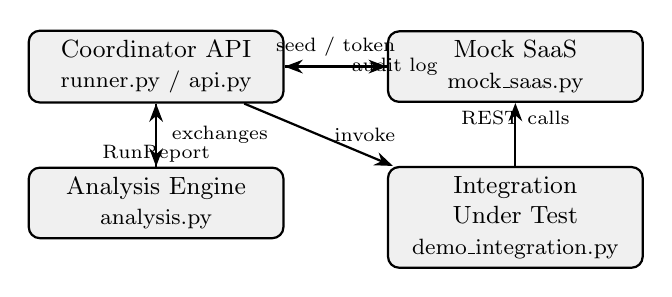
\begin{tikzpicture}[node distance=0.45cm and 1.1cm]
    \node[svcbox] (coord) {Coordinator API\\{\footnotesize runner.py / api.py}};
    \node[svcbox, right=1.3cm of coord] (mock) {Mock SaaS\\{\footnotesize mock\_saas.py}};
    \node[svcbox, below=0.8cm of mock] (iut) {Integration\\Under Test\\{\footnotesize demo\_integration.py}};
    \node[svcbox, below=0.8cm of coord] (ae) {Analysis Engine\\{\footnotesize analysis.py}};
    \draw[arrow] (coord) -- node[above,font=\scriptsize]{seed / token} (mock);
    \draw[arrow] (coord) -- node[right,font=\scriptsize,xshift=2pt]{invoke} (iut);
    \draw[arrow] (iut)   -- node[above,font=\scriptsize]{REST calls} (mock);
    \draw[arrow] (mock)  -- node[right,font=\scriptsize,xshift=2pt]{audit log} (coord);
    \draw[arrow] (coord) -- node[right,font=\scriptsize,xshift=2pt]{exchanges} (ae);
    \draw[arrow] (ae)    -- node[below,font=\scriptsize]{RunReport} (coord);
  \end{tikzpicture}
  \caption{AIT system architecture. Arrows show data flow direction.}
  \label{fig:arch}
\end{figure}

\subsection{Coordinator API}

The Coordinator exposes \texttt{POST /runs} and
\texttt{GET /runs/\{run\_id\}}. On invocation it: generates a unique
12-character hexadecimal \texttt{run\_id}; resolves an OAuth token;
seeds the Mock SaaS with taint data; invokes the IUT under baseline
and mutated conditions; retrieves the audit log; and forwards
exchanges to the Analysis Engine. \texttt{TargetConfig} objects
encode the security policy: \texttt{expected\_endpoints},
\texttt{expected\_scopes}, and \texttt{sensitive\_markers}.
Figure~\ref{fig:pipeline} sketches how recorded traffic flows into the
Analysis Engine and structured findings.

\subsection{Mock SaaS Service}

The Mock SaaS retains the original CRM surface
(\texttt{/api/v1/customers}, \texttt{/customers/\{id\}},
\texttt{/customers/\{id\}/notes}, \texttt{/customers/\{id\}/billing})
for mechanism-isolation experiments (Section~\ref{sec:eval}).
The billing endpoint is omitted from \texttt{expected\_endpoints} but
accessible via the over-provisioned scope, instantiating capabilities
C1 and~C2 on that surface.
Administrative routes (\texttt{/oauth/token}, \texttt{/admin/seed},
\texttt{/admin/audit/\{run\_id\}}) support the Coordinator. In
addition, the service exposes \emph{platform-inspired} REST paths
patterned after Slack, GitHub, Google Gmail, Notion, and Trello (e.g.,
channel history, repository listings, mail send, page updates, and
card creation). Synthetic responses are written to the same structured
audit log consumed by the Analysis Engine, so DM1--DM3 operate
uniformly across both the CRM corpus and the extended corpus.

\subsection{Live SaaS Runner}

The \texttt{ait/live\_runner.py} module implements a direct evaluation
path for explicit sandbox scenarios. It reads bearer tokens from
environment variables, executes operator-defined baseline and mutated
requests against real SaaS APIs (e.g., \texttt{api.github.com},
\texttt{api.notion.com}), converts HTTP responses into
\texttt{CapturedExchange} records without mock-side instrumentation,
and adds policy findings when a request expected to be denied succeeds
or vice versa. The \texttt{generate\_live\_saas\_results.py} script
loads YAML scenario files from \texttt{live\_test\_cases/}, executes
them, and writes structured artifacts to \texttt{results/live\_saas/}
for downstream analysis. Operational guidance (use only accounts you
control; stay within rate limits; do not commit tokens) is enforced
via \texttt{.gitignore} and documented in
\texttt{docs/LIVE\_SAAS\_EVALUATION.md}.

\subsection{Analysis Engine and Data Model}

The Analysis Engine applies four detection mechanisms to
\texttt{CapturedExchange} objects and produces a \texttt{RunReport}
with \texttt{Finding} objects and a risk score. All data is typed via
Pydantic~v2 models, enabling deterministic JSON serialization and
downstream SIEM ingestion.

\begin{figure}[htbp]
  \centering
  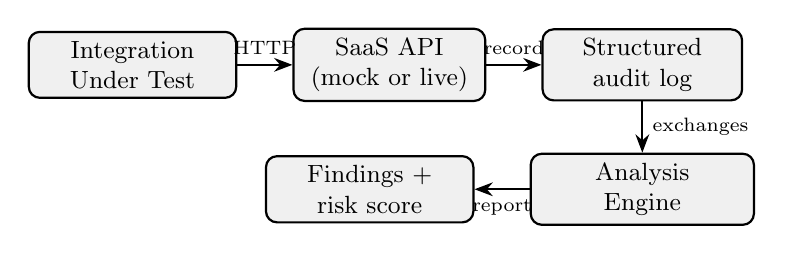
\begin{tikzpicture}[node distance=0.35cm and 0.55cm, font=\small]
    \node[svcbox, text width=2.4cm] (iut) {Integration\\Under Test};
    \node[svcbox, right=0.7cm of iut, text width=2.2cm] (api) {SaaS API\\(mock or live)};
    \node[svcbox, right=0.7cm of api, text width=2.3cm] (log) {Structured\\audit log};
    \node[svcbox, below=0.65cm of log, text width=2.6cm] (ae) {Analysis\\Engine};
    \node[svcbox, left=0.7cm of ae, text width=2.4cm] (rep) {Findings +\\risk score};
    \draw[arrow] (iut) -- node[above,font=\scriptsize]{HTTP} (api);
    \draw[arrow] (api) -- node[above,font=\scriptsize]{record} (log);
    \draw[arrow] (log) -- node[right,font=\scriptsize]{exchanges} (ae);
    \draw[arrow] (ae) -- node[below,font=\scriptsize]{report} (rep);
  \end{tikzpicture}
  \caption{End-to-end detection pipeline: observed integration traffic is
  normalized into \texttt{CapturedExchange} records, analyzed against
  policy, and emitted as structured findings. The same pipeline is used
  for both mock and live evaluations.}
  \label{fig:pipeline}
\end{figure}

% -------------------------------------------------------
\section{Methodology}
\label{sec:method}

\subsection{Dual-Phase Execution Model}

Fig.~\ref{fig:dualphase} illustrates the dual-phase flow, designed
to address adversary capability C3. Two execution phases differ only
in the state signal sent to the IUT:

\begin{figure}[htbp]
  \centering
  \begin{tikzpicture}[node distance=0.5cm and 0.9cm, font=\small]
    \node[svcbox, text width=2.5cm] (start) {Coordinator\\initiates run};
    \node[phase, below=0.6cm of start, text width=6.8cm] (bp) {
      \textbf{Baseline Phase} \\[2pt]
      \begin{tikzpicture}[node distance=0.35cm]
        \node[svcbox, text width=2.0cm] (b1) {Invoke IUT\\(normal state)};
        \node[svcbox, right=0.5cm of b1, text width=2.2cm] (b2) {Log calls\\label=``baseline''};
        \draw[arrow] (b1) -- (b2);
      \end{tikzpicture}
    };
    \node[phase, below=0.5cm of bp, text width=6.8cm] (mp) {
      \textbf{Mutated Phase} \\[2pt]
      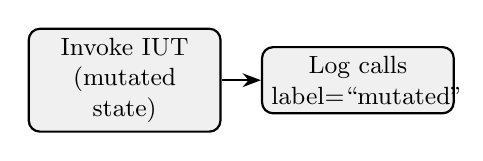
\begin{tikzpicture}[node distance=0.35cm]
        \node[svcbox, text width=2.2cm] (m1) {Invoke IUT\\(mutated state)};
        \node[svcbox, right=0.5cm of m1, text width=2.2cm] (m2) {Log calls\\label=``mutated''};
        \draw[arrow] (m1) -- (m2);
      \end{tikzpicture}
    };
    \node[svcbox, below=0.6cm of mp, text width=2.8cm] (ae2)
      {Analysis Engine:\\compute divergence};
    \draw[arrow] (start) -- (bp);
    \draw[arrow] (bp)    -- (mp);
    \draw[arrow] (mp)    -- (ae2);
  \end{tikzpicture}
  \caption{Dual-phase execution. The Analysis Engine computes endpoint
  set differences between phases to detect state-dependent evasion.}
  \label{fig:dualphase}
\end{figure}

\textbf{Baseline Phase:} Integration invoked under normal state; all
API calls recorded with label \texttt{"baseline"}.

\textbf{Mutated Phase:} Integration invoked with
\texttt{phase="mutated"}, activating feature flags or latent branches;
calls recorded with label \texttt{"mutated"}.

Endpoints in the mutated set but not the baseline set signal
state-dependent behavior that may conceal unauthorized access.

\subsection{Taint-Seeded Data Tracking}

Before each run, \texttt{POST /admin/seed} updates sensitive fields in
Mock SaaS records with run-specific synthetic tokens (e.g.,
\texttt{billing\_email = \{run\_id\}@example.test}). These values are
globally unique, contain no real user data, and serve two roles:
(i)~taint injection, enabling response-level detection of sensitive
field access; and (ii)~run attribution, ensuring concurrent test runs
cannot contaminate one another's audit records. No IUT instrumentation
is required. In the live SaaS runner, sensitive markers are checked
against actual API response payloads; real credentials or PII in
responses are never logged in plaintext.

\subsection{Detection Mechanisms}

\textbf{DM1 --- Hidden Endpoint Detection} (addresses C1):
\begin{equation}
  H = R \setminus E
  \label{eq:hidden}
\end{equation}
where $R$ = reached endpoints, $E$ = expected endpoints. Each $h \in H$
yields a \texttt{HIGH}-severity \texttt{HIDDEN\_ENDPOINT} finding.

\textbf{DM2 --- Sensitive Field Access Detection} (addresses C2):
Any \texttt{CapturedExchange} where \texttt{contains\_sensitive\_marker}
is true or response fields intersect \texttt{sensitive\_markers} yields
a \texttt{CRITICAL}-severity \texttt{SENSITIVE\_FIELD\_ACCESS} finding.

\textbf{DM3 --- Behavioral Divergence Detection} (addresses C3):
\begin{equation}
  D = M \setminus B
  \label{eq:divergence}
\end{equation}
where $M$ = mutated-phase endpoint set, $B$ = baseline-phase endpoint
set. Non-empty $D$ yields a \texttt{HIGH}-severity
\texttt{BEHAVIORAL\_DIVERGENCE} finding.

Allow/deny expectation checks against live HTTP status codes are
\emph{out of scope} for the current release (future work); the live
runner today reuses DM1--DM3 on captured exchanges only.

\subsection{Informal Detection Guarantees}

Under black-box observation of traffic recorded in the audit log and
relative to a supplied \texttt{TargetConfig}, AIT \emph{reports}:
(G1)~any reached path outside \texttt{expected\_endpoints};
(G2)~responses whose extracted fields intersect \texttt{sensitive\_markers}
(or carry the synthetic taint flag); and (G3)~phase-specific endpoint-set
differences consistent with Eq.~\eqref{eq:divergence}.
These are sound \emph{with respect to the observed run}---they do not
prove absence of violations outside the logged surface. AIT
\emph{does not} guarantee detection of FN1--FN4
(Section~\ref{sec:fn}): out-of-band exfiltration, shared-token misuse,
delayed activation, or field-name aliasing beyond configured markers.

\subsection{Risk Scoring Model}

\begin{equation}
  S = \min\!\bigl(100,\;
        w_H \cdot |H| + w_F \cdot |F_s| + w_D \cdot |D|
      \bigr)
  \label{eq:risk}
\end{equation}

Weights $(w_H, w_F, w_D) = (25, 20, 15)$ are \emph{heuristic design
constants} inspired by the CVSS~v3.1 severity taxonomy~\cite{cvss31}
(not empirically calibrated scores): C1 maps to
Scope:Changed/Confidentiality:High (base score 7.5--9.0, $w_H=25$);
C2 maps to Confidentiality:High without scope change (6.5--7.5,
$w_F=20$); C3 represents architectural risk without confirmed data
access (4.0--6.0, $w_D=15$). Score bands: 0--25 (Low), 26--50
(Medium), 51--75 (High), 76--100 (Critical).

The scoring model is a \emph{triage signal}, consistent with CVSS's
own stated intent as an approximation rather than a precise
measurement. Empirical calibration against a ground-truth dataset of
real integration violations is identified as future work.

% -------------------------------------------------------
\section{Implementation}
\label{sec:impl}

\subsection{Technology Stack}

AIT uses Python~3.11+, FastAPI, \texttt{asyncio}/\texttt{httpx},
Pydantic~v2, and \texttt{uvicorn} across three processes on ports
8000--8002. Test policies are YAML files validated against the
\texttt{TargetConfig} schema. The paper-results generator
(\texttt{generate\_paper\_results.py}) runs mock and integration apps
in-process via ASGI transports rather than spawning external processes,
enabling fully deterministic execution without network dependencies.
The live results generator (\texttt{generate\_live\_saas\_results.py})
issues real HTTP requests to provider APIs and writes structured
artifacts to \texttt{results/live\_saas/}. All scenario definitions,
expected categories, and attack paths are stored in YAML \texttt{paper:}
metadata blocks, allowing reported tables to be regenerated
bit-for-bit given a fixed software version.

\subsection{Assessment Execution Flow}

A representative non-measured example sequence for a mock assessment is:
token resolution, taint seeding, baseline invocation (declared API
calls), mutated invocation (including optional over-scope paths), audit
retrieval, analysis, and report return. Wall-clock timings for this
sequence are \emph{not claimed} here; measured Analysis Engine
latencies appear only in the generated benchmark table.
Live assessments are expected to be
dominated by WAN latency; measured GitHub/Notion sandbox timings are
\texttt{NOT RUN} (Task~6 blocked without credentials).

\subsection{Practical Deployment Considerations}
\label{sec:deployment}

Several engineering challenges arise when deploying AIT beyond the
mock environment. A practical pattern is to run AIT from CI/CD before
shipping an integration change: failures gate merges when new endpoints
or sensitive markers appear relative to the checked-in policy YAML.

\begin{figure}[htbp]
  \centering
  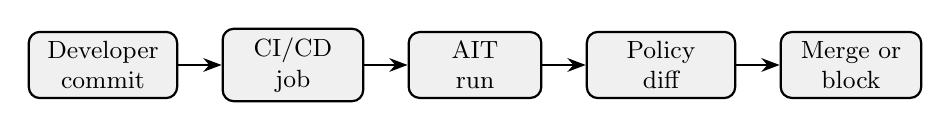
\begin{tikzpicture}[node distance=0.35cm and 0.5cm, font=\footnotesize]
    \node[svcbox, text width=1.65cm] (dev) {Developer\\commit};
    \node[svcbox, right=0.55cm of dev, text width=1.55cm] (cicd) {CI/CD\\job};
    \node[svcbox, right=0.55cm of cicd, text width=1.45cm] (ait) {AIT\\run};
    \node[svcbox, right=0.55cm of ait, text width=1.65cm] (pol) {Policy\\diff};
    \node[svcbox, right=0.55cm of pol, text width=1.55cm] (gate) {Merge or\\block};
    \draw[arrow] (dev) -- (cicd);
    \draw[arrow] (cicd) -- (ait);
    \draw[arrow] (ait) -- (pol);
    \draw[arrow] (pol) -- (gate);
  \end{tikzpicture}
  \caption{Deployment sketch: integration changes are gated on AIT policy
  reconciliation before release.}
  \label{fig:cicd}
\end{figure}

\emph{OAuth flow heterogeneity:} production platforms
differ significantly in token issuance, scope granularity, and
refresh semantics; AIT's \texttt{TargetConfig} is designed to be
platform-parameterizable, but per-platform adapters are required.
The live runner currently supports bearer-style tokens, covering
GitHub PATs, Notion integration tokens, Slack bot tokens, and
Google access tokens; platforms with non-bearer auth conventions
require a small adapter.
\emph{Rate limiting:} live SaaS APIs enforce request limits; a
production Coordinator must implement exponential backoff and
respect \texttt{Retry-After} headers. \emph{Audit log availability:}
not all SaaS platforms expose structured audit logs to third parties;
AIT may require proxy-mode interception in such cases.
\emph{Scalability:} the current in-memory store is unsuitable for
concurrent runs at scale; a production backend (PostgreSQL or Redis)
is required. \emph{Integration overhead:} each AIT run issues
$\mathcal{O}(N_e)$ additional HTTP requests where $N_e$ is the
number of endpoints under test; for large API surfaces this may
require phased execution.

\subsection{Report Generation}

AIT produces \emph{structured JSON} (for CI/CD and SIEM ingestion)
and \emph{HTML} (color-coded findings, endpoint access matrices, and
per-finding remediation guidance) deterministically from the same
\texttt{RunReport}. The paper-results pipeline additionally writes
\texttt{detection\_metrics.csv} (per-category TP/FP/FN, precision,
recall, F1), \texttt{summary.json} (aggregate counts and score
ranges), and \texttt{paper\_snippets.md} (paper-ready markdown
derived from the generated metrics). Live results are written to
\texttt{results/live\_saas/} and include a \texttt{results\_table.csv},
\texttt{summary.json}, \texttt{skipped.json}, and
\texttt{raw\_run\_artifacts.json}; the last file is \texttt{.gitignore}d
to prevent accidental commitment of real account metadata.

% -------------------------------------------------------
\section{Experimental Evaluation}
\label{sec:eval}

\subsection{Evaluation Design and Scope}
\label{sec:evalscope}

The evaluation has five components: (1)~controlled mock-environment
experiments over a 16-scenario offline corpus---6~CRM scenarios
(3~isolation cases plus 3~compliant controls) and 10~platform-inspired
mocks (7~violation-oriented cases plus 3~compliant controls);
(2)~a live SaaS evaluation pipeline for explicit sandbox scenarios against
real provider APIs (GitHub and Notion; empirical rows \texttt{NOT RUN}/BLOCKED
without credentials); (3)~a read-only GitHub REST
smoke probe plan under an explicit allowlist policy; (4)~a tool capability
comparison with RESTler and EvoMaster; and (5)~a log-based replay
experiment applying AIT's detection logic to researcher-constructed traces
from public disclosures.
Components~(1)--(3) provide increasing levels of evidence from fully
controlled conditions toward live vendor REST traffic; live empirical
anchors remain pending Task~6. Component~(5)
provides an alignment signal on reconstructed disclosures. Together they mitigate the
concern that mock-only evaluation lacks any live-surface design path.
Limitations of each component are explicitly stated. All mock
experiments are reproducible via version-controlled YAML scenarios and
deterministic in-process execution pipelines.

\subsection{Mock Environment: Test Scenarios}

Three CRM isolation scenarios separate detection mechanisms; three additional
CRM controls exercise compliant baselines (6~CRM total):

\begin{itemize}
  \item \textbf{S1 --- C1 only:} IUT accesses billing endpoint in
        both phases; no taint configured.
  \item \textbf{S2 --- C2 only:} IUT accesses only declared endpoints;
        responses contain tainted field values.
  \item \textbf{S3 --- C1 + C2 + C3 combined:} IUT accesses billing
        in the mutated phase only, with tainted \texttt{billing\_email}
        and \texttt{tax\_id}.
\end{itemize}

\subsection{Mock Environment: Detection Results}

% CLAIM:mock-overall-f1
% CLAIM:mock-category-metrics
Table~\ref{tab:results} reports precision (P), recall (R), and F1 per
finding category with TP/FP/FN denominators over the offline scenario
corpus (CRM and platform-inspired mocks). A finding is a true positive
if it correctly identifies a known-injected violation; false positive if
it fires on a non-violation; false negative if it misses a known
violation. Values are regenerated from
\texttt{results/derived/scenario\_metrics.json}.

\begin{table}[htbp]
  \caption{Detection Performance, Offline Mock Corpus (category metrics
  with micro-average; implementation validation under injected labels)}
  \label{tab:results}
  \centering
  \renewcommand{\arraystretch}{1.25}
  \footnotesize
  \input{results/generated/mock_detection_results.tex}
\end{table}

\noindent\textit{Takeaway:} Under injected labels, AIT's implementation
matches the intended DM1--DM3 logic on this controlled corpus.

\noindent\textit{Interpretation note:} Perfect controlled scores, when
observed, validate that the implementation executes the defined
detection logic---not that the system generalizes to unseen or
adversarial inputs. External validity requires live platform evaluation
(Section~\ref{sec:livesaas} and future work, Section~\ref{sec:future}).

\subsection{Platform-Inspired Mock Suite}
\label{sec:platformmock}

Beyond the minimal CRM surface used to \emph{isolate} DM1--DM3
(Section~\ref{sec:eval}), we extended the Mock SaaS and Integration
Under Test with additional REST paths \emph{inspired by} five major
SaaS ecosystems---Slack, GitHub, Google Gmail, Notion, and Trello---each
exercising a distinct over-permissioning idiom (hidden history access,
private-repository fields under nominally public scope, write calls
under read-only mode, content updates under read-only integration
assumptions, and mutating write behavior under read-scoped tokens).
Two additional integrations are \emph{compliant baselines} included
to probe false positives.

\noindent\textbf{Important framing:} These paths are \emph{synthetic
mocks} for controlled evaluation; they are not claims of measurement
on vendor production APIs. External validity is addressed in part by
the live SaaS evaluation (Section~\ref{sec:livesaas}) and remains
a priority for future work (Section~\ref{sec:future}).

Each scenario is specified as a YAML \texttt{TargetConfig} (declared
scopes, expected endpoint allowlist, sensitive markers) and executed
through the same Coordinator pipeline as the CRM suite. Risk scores
follow Eq.~\eqref{eq:risk} with $(w_H,w_F,w_D)=(25,20,15)$.

% CLAIM:platform-scenario-risks
\begin{table}[htbp]
  \caption{Platform-Inspired Mock Results (risk scores from offline
  scenario artifacts; synthetic mocks, not vendor production APIs)}
  \label{tab:platform}
  \centering
  \renewcommand{\arraystretch}{1.2}
  \footnotesize
  \setlength{\tabcolsep}{3pt}
  \input{results/generated/platform_scenario_results.tex}
\end{table}

\noindent\textit{Takeaway:} AIT maintains detection on heterogeneous
platform-inspired mock idioms while reporting zero risk on the
compliant baselines included in the generated table.

\noindent\textbf{Interpretation:} As with Table~\ref{tab:results},
perfect agreement with declared labels on this deterministic corpus
validates end-to-end wiring and reporting across multiple API idioms,
not generalization to arbitrary production tenants.

\subsection{Live SaaS Evaluation}
\label{sec:livesaas}

To bridge the gap between controlled mock evaluation and real platform
behavior, AIT provides an instrumented live probe runner
(\texttt{ait/live\_runner.py}) for sandbox accounts using read-only
tokens from environment variables. Plans under \texttt{configs/live/}
specify base URL, declared endpoints, and request sequences. Real
sandbox Task~6 execution is \textbf{BLOCKED} without credentials and
is recorded as \texttt{NOT RUN}; no fabricated live observations are
substituted.

\noindent\textbf{GitHub sandbox:} Declared read-only probe design
(allowlisted hosts/paths; policy mismatch detection when undeclared
surfaces are reached). Empirical result: \texttt{NOT RUN} (blocked).

\noindent\textbf{Notion sandbox:} Declared read-path validation design
(\texttt{GET /v1/users/me}). Empirical result: \texttt{NOT RUN} (blocked).

% Live rows are generated; artifact currently null → NOT RUN (claim optional).
\begin{table}[htbp]
  \caption{Live SaaS Evaluation Results (Sandbox Accounts;
  unavailable artifacts render as \texttt{NOT RUN})}
  \label{tab:live}
  \centering
  \renewcommand{\arraystretch}{1.2}
  \footnotesize
  \setlength{\tabcolsep}{3pt}
  \input{results/generated/live_results.tex}
\end{table}

\noindent\textit{Takeaway:} Live sandbox rows remain unavailable until
Task~6 completes with real credentials and redacted artifacts. Design
coverage (positive and negative control plans) is in place; empirical
claims await those artifacts.

\noindent\textit{Interpretation note:} When live results exist, a
positive GitHub finding would indicate the supplied token's actual
capabilities exceeded the declared policy---a policy mismatch in the
evaluation setup, not a vulnerability in the GitHub platform. No live
durations are reported here (\texttt{NOT RUN}).

\subsection{Live GitHub REST Smoke Probe (Optional)}
\label{sec:livegithub}

Complementing the structured sandbox plans in
Section~\ref{sec:livesaas}, a separate read-only probe is defined to
exercise \texttt{api.github.com} under a stricter policy allowlisting only
\texttt{/user}, with additional undeclared \texttt{/user/repos} and
\texttt{/user/orgs} requests. Empirical smoke-probe results remain
\texttt{NOT RUN} until a hashed live artifact is selected in
\texttt{configs/paper\_artifacts.yaml}. When executed with a read-only
PAT via \texttt{AIT\_GITHUB\_TOKEN}, the signal of interest is
\emph{policy mismatch}, not server-side exploitability.

\subsection{Robustness and Noise}
\label{sec:robust}

% CLAIM:robustness-suite
% CLAIM:reproducibility-5
To move beyond purely ``clean'' traces, the repository includes
robustness and evasion scenario YAML (noise, partial exposure, path
ambiguity, FN4 field-alias negatives, and model-boundary cases).
Table~\ref{tab:robust} reports suite status from the selected
\texttt{robustness\_metrics} artifact required by the offline release gate
(\texttt{robustness\_results}). Deterministic reproducibility across five
repetitions is recorded in the hashed \texttt{reproducibility} artifact.

\begin{table}[htbp]
  \caption{Robustness / Evasion Suite Status}
  \label{tab:robust}
  \centering
  \renewcommand{\arraystretch}{1.2}
  \input{results/generated/robustness_results.tex}
\end{table}

\subsection{Scalability of Analysis}
\label{sec:scale}

% CLAIM:benchmark-timings
\noindent\textbf{Isolation note:} This micro-benchmark measures Analysis
Engine latency only; full end-to-end Coordinator runs remain dominated
by network I/O and OAuth/token work; live SaaS
timings in Section~\ref{sec:livesaas} are \texttt{NOT RUN}.

Table~\ref{tab:scale} reports median, p95, and MAD wall time from the
hashed offline benchmark artifact (warmups and repetitions recorded in
provenance). Risk scores are taken from the same synthetic-log
protocol.

\begin{table}[htbp]
  \caption{Analysis Engine Micro-Benchmark (Synthetic Log Width;
  median/p95/MAD from offline \texttt{benchmark\_summary} artifact)}
  \label{tab:scale}
  \centering
  \renewcommand{\arraystretch}{1.2}
  \footnotesize
  \input{results/generated/benchmark_results.tex}
\end{table}

\noindent\textit{Takeaway:} Detection output is stable as synthetic log
width grows within this micro-benchmark; analysis time does not reflect
WAN latency.

\subsection{Tool Capability Comparison}
\label{sec:toolcompeval}

RESTler and EvoMaster target complementary server-side fault classes.
A pinned Docker comparison protocol lives under \texttt{comparison/};
until a hashed \texttt{tool\_comparison} artifact is selected,
Table~\ref{tab:comparison} reports \texttt{NOT RUN} rather than
invented detection outcomes. Do not interpret absence as ``no findings.''

\begin{table}[htbp]
  \caption{Tool Capability Comparison (selected artifact or
  \texttt{NOT RUN})}
  \label{tab:comparison}
  \centering
  \renewcommand{\arraystretch}{1.25}
  \input{results/generated/tool_comparison.tex}
\end{table}

\noindent\textit{Takeaway:} When executed, the taxonomy is intended to
clarify complementary deployment: server fuzzers for implementation bugs,
AIT for integration policy drift. No external-tool run is claimed here.

\subsection{Log-Based Replay: Researcher-Constructed Traces}
\label{sec:replay}

% CLAIM:replay-exact-match
To provide an alignment signal without requiring live
platform credentials, we conducted a log-based replay experiment.
Public post-mortem disclosures from three documented SaaS security
incidents---CircleCI (2023)~\cite{circleci2023},
Okta (2022)~\cite{okta2022}, and the GitHub OAuth token
exposure (2022)~\cite{github2022}---were manually reconstructed into
\texttt{CapturedExchange} sequences (researcher-constructed traces from
public disclosures, not ground-truth API logs). These traces were fed
to AIT's Analysis Engine and compared against expected categories.
Table~\ref{tab:replay} is regenerated from the hashed replay artifact.

\begin{table}[htbp]
  \caption{Log-Based Replay: Expected vs.\ Observed Categories
  (researcher-constructed traces)}
  \label{tab:replay}
  \centering
  \renewcommand{\arraystretch}{1.25}
  \footnotesize
  \input{results/generated/replay_results.tex}
\end{table}

\noindent\textit{Takeaway:} Replay provides \emph{plausibility evidence}
that AIT's detection categories map to independently reported incident
classes, not empirical precision/recall on real platform data.

\subsection{Risk Score and Sensitivity Analysis}

% CLAIM:risk-sensitivity-bands
Under the default weights $(w_H,w_F,w_D)=(25,20,15)$, multi-finding
scenarios can enter the Critical band ($>75$). Table~\ref{tab:sensitivity}
reports $\pm30\%$ single-weight perturbations for selected CRM scenarios
from the hashed sensitivity artifact.

\begin{table}[htbp]
  \caption{Risk Score Sensitivity ($\pm30\%$ Weight Variation;
  selected CRM scenarios from offline artifacts)}
  \label{tab:sensitivity}
  \centering
  \renewcommand{\arraystretch}{1.25}
  \footnotesize
  \input{results/generated/risk_sensitivity.tex}
\end{table}

Band transitions, when present, are recorded in
\texttt{sensitivity\_summary}; the score remains a triage signal, not a
precise risk measurement.

% CLAIM:artifact-provenance
\subsection{Artifact Provenance}

Table~\ref{tab:provenance} lists the selected paper artifacts and
SHA-256 prefixes used for this compilation.

\begin{table}[htbp]
  \caption{Selected Artifact Provenance}
  \label{tab:provenance}
  \centering
  \renewcommand{\arraystretch}{1.2}
  \footnotesize
  \input{results/generated/artifact_provenance.tex}
\end{table}

\subsection{Discussion}

The dual-phase model correctly differentiated baseline behavior
(three authorized endpoints) from mutated behavior (four endpoints
including one unauthorized). Static audits miss the key distinction here:
the billing call was \emph{OAuth-authorized} yet \emph{policy-violating}
under the declared allowlist. The live SaaS evaluation (Table~\ref{tab:live})
is designed to provide the same detection path on live vendor APIs, but
empirical sandbox rows remain \texttt{NOT RUN}/\textbf{BLOCKED} without
credentials.
Replay and platform mocks (Table~\ref{tab:platform}) support that
C1--C3 map to realistic abuse shapes without changing core detection
rules. AIT's value lies not in replacing existing tools but in
introducing a missing verification layer between declared policy and
observed behavior.

% -------------------------------------------------------
\section{False Negative Analysis}
\label{sec:fn}

A rigorous analysis of cases where AIT will fail to detect a violation
is essential to characterize the security guarantees of the framework.
Four evasion scenarios are identified:

\textbf{FN1 --- Out-of-Band Exfiltration.} An integration that accesses
authorized endpoints but exfiltrates data via a separate webhook,
outbound HTTP request, or side channel will not be detected, as AIT
observes only inbound API calls to the instrumented SaaS surface.
\emph{Mitigation direction:} network egress monitoring or outbound
traffic analysis, out of scope for the current framework.

\textbf{FN2 --- Shared Token Misuse.} If two integrations share an
OAuth token issued to a different client ID, AIT---which attributes
calls by run ID, not token identity---will not associate the
unauthorized calls with the IUT. \emph{Mitigation direction:}
per-integration token isolation at the platform level.

\textbf{FN3 --- Time-Delayed or Trigger-Based Activation.} An
integration that activates unauthorized access after a fixed delay
(e.g., 30~days post-installation) or via an external command-and-control
signal will evade the two-phase model, which is bounded by the test
session duration. \emph{Mitigation direction:} continuous runtime
monitoring beyond point-in-time assessment.

\textbf{FN4 --- Response-Field Aliasing.} If an integration reads
sensitive data from a field whose name does not match any token in
\texttt{sensitive\_markers} (e.g., a renamed or obfuscated field in
a non-standard API response schema), taint detection will fail.
\emph{Mitigation direction:} value-pattern matching in addition to
field-name matching; semantic field classification using NLP.
The mock harness reproduces this miss explicitly (Section~\ref{sec:robust},
FN4 negative row).

These false negative cases are not implementation bugs but fundamental
constraints of the black-box, session-bounded, field-name-based
detection model. Acknowledging them explicitly bounds the framework's
security guarantees and scopes the threat model accurately.

% -------------------------------------------------------
\section{Limitations and Future Work}
\label{sec:limit}

\subsection{Current Limitations}

\textbf{External Validity:} Primary evidence comprises mock scenarios,
replayed public incidents, and a live probe design for two sandbox
accounts (GitHub and Notion) whose Task~6 empirical rows are
\texttt{NOT RUN}/\textbf{BLOCKED} without credentials. The framework has not been
evaluated tenant-wide on live production SaaS platforms; this remains
the primary limitation.

\textbf{Evaluation Scale:} The offline mock corpus comprises 16~YAML
scenarios: 6~CRM (3~isolation + 3~controls) and 10~platform-inspired
(7~violation-oriented + 3~compliant controls). Live sandbox plans exist
but empirical runs are blocked.
Together they
remain a finite corpus and do not explore all edge cases, adversarial
inputs, or unexpected API behavior. A larger, more adversarial test
suite is needed.

\textbf{Scoring Model:} The heuristic design-constant weights are justified and
sensitivity-analyzed, but not empirically validated against a
ground-truth dataset of real integration violations. Allow/deny live
policy checks (and any associated score addends) remain future work /
not yet implemented.

\textbf{Two-Phase Model:} Real integrations may exhibit variation
across more state dimensions than two phases can capture
(Section~\ref{sec:fn}, FN3).

\textbf{In-Memory State:} Non-persistent and not multi-process safe;
a production deployment requires a persistent backend.

\textbf{Live Runner Auth:} The current bearer-token auth shape covers
GitHub, Notion, Slack, and Google; platforms with non-standard auth
conventions (query-param tokens, multi-step flows) require per-platform
adapters before evaluation.

\subsection{Future Work}
\label{sec:future}

\begin{enumerate}
  \item \emph{Live platform evaluation} against Slack, GitHub, and
        Google Workspace sandbox accounts at broader scale---the
        single highest-impact next step.
  \item \emph{Automatic policy inference} from OpenAPI specifications
        and historical access logs.
  \item \emph{ML-based anomaly detection} for access patterns not
        requiring pre-specified allowlists.
  \item \emph{Multi-phase state-machine-guided execution} to cover
        richer behavioral spaces.
  \item \emph{Outbound traffic monitoring} to address FN1
        (out-of-band exfiltration).
  \item \emph{Value-pattern taint matching} to address FN4
        (response-field aliasing).
  \item \emph{CI/CD pipeline integration} for automated regression
        testing on each integration deployment.
  \item \emph{Empirical risk-weight calibration} against a labeled
        dataset of real integration violations.
\end{enumerate}

% -------------------------------------------------------
\section{Conclusion}
\label{sec:conc}

AIT closes a gap left by server-focused fuzzers and static scope tools:
black-box reconciliation of observed integration traffic against an
explicit policy artifact. The design combines an \emph{integration-centric}
test subject, \emph{dual-phase} stimulation for C3, and
\emph{instrumentation-free} taint markers for C2. A live SaaS
evaluation pipeline (\texttt{ait/live\_runner.py}) is implemented for
instrumented sandbox probes, but GitHub and Notion Task~6 results remain
\texttt{NOT RUN}/\textbf{BLOCKED} without credentials---no live risk
scores are claimed.

Claims are scoped to controlled mocks, live sandbox evaluations,
optional smoke probes, and replayed public incidents; false-negative
analysis bounds guarantees. Broader tenant-scale validation remains
future work. This work establishes \emph{integration-policy conformance}
as a first-class security property in SaaS ecosystems. AIT enables
organizations to verify integration behavior before and after deployment
(Fig.~\ref{fig:cicd}), tightening least-privilege practice under
zero-trust assumptions.

% -------------------------------------------------------
\section*{Acknowledgment}

The authors thank the Department of CSE (IoT \& Cybersecurity
Including Blockchain Technology), Bangalore Institute of Technology,
for supporting this work under Major Project Phase~1 (BIC685).

% -------------------------------------------------------
\begin{thebibliography}{35}

\bibitem{csa2023}
Cloud Security Alliance, ``SaaS Security Survey Report,'' 2023.

\bibitem{solarwinds2020}
CISA, ``Alert (AA20-352A): Advanced Persistent Threat Compromise of
Government Agencies, Critical Infrastructure, and Private Sector
Organizations,'' Dec.~2020.

\bibitem{okta2022}
Okta, ``Okta Security Incident: January~2022,'' Security Advisory,
Mar.~2022.

\bibitem{circleci2023}
CircleCI, ``CircleCI Security Incident Disclosure and Recommended
Customer Actions,'' Jan.~2023. [Online]. Available:
\url{https://circleci.com/blog/jan-4-2023-security-alert/}

\bibitem{github2022}
GitHub, ``Security Alert: Attack Campaign Involving Stolen OAuth
User Tokens Issued to Two Third-Party Integrators,'' Apr.~2022.
[Online]. Available:
\url{https://github.blog/2022-04-15-security-alert-stolen-oauth-user-tokens/}

\bibitem{aliyu2023}
F.~Aliyu, C.~Benson, and M.~Ismail, ``Over-Privileged OAuth Grants
in Enterprise SaaS: Measurement and Risk Characterization,''
\textit{IEEE Trans.\ Dependable Secure Comput.}, vol.~20, no.~4,
pp.~3211--3225, Jul./Aug.~2023.

\bibitem{rfc6749}
D.~Hardt, Ed., ``The OAuth 2.0 Authorization Framework,'' RFC~6749,
IETF, Oct.~2012.

\bibitem{rfc7636}
N.~Sakimura, J.~Bradley, and N.~Agarwal, ``Proof Key for Code
Exchange by OAuth Public Clients,'' RFC~7636, IETF, Sep.~2015.

\bibitem{oidc}
N.~Sakimura et al., ``OpenID Connect Core 1.0,'' OpenID Foundation,
Nov.~2014. [Online]. Available: \url{https://openid.net/connect/}

\bibitem{fett2017}
D.~Fett, R.~K\"{u}sters, and G.~Schmitz, ``The Web SSO Standard
OpenID Connect: In-Depth Formal Security Analysis and Security
Guidelines,'' \textit{Proc.\ IEEE CSF}, 2017.

\bibitem{felt2012}
A.~P. Felt, E.~Ha, S.~Egelman, A.~Haney, E.~Chin, and D.~Wagner,
``Android Permissions: User Attention, Comprehension, and Behavior,''
\textit{Proc.\ SOUPS}, 2012.

\bibitem{owasp2023}
OWASP, ``OWASP API Security Top 10 -- 2023 Edition.'' [Online].
Available: \url{https://owasp.org/www-project-api-security/}

\bibitem{mainka2022}
C.~Mainka, V.~Mladenov, J.~Schwenk, and T.~Wich, ``SoK: Benchmarking
the Effectiveness of OAuth Grant Type Enforcement Across Major SaaS
Providers,'' \textit{Proc.\ ACM CCS}, 2022.

\bibitem{decarne2023}
X.~De Carné de Carnavalet and P.~C. van Oorschot, ``Third-Party
Application Permission Practices: A Large-Scale Analysis of OAuth
over Major Identity Providers,'' \textit{Proc.\ USENIX Security},
2023.

\bibitem{boucher2024}
T.~Boucher, A.~Kharraz, and E.~Kirda, ``Scope Guard: Static Policy
Enforcement for SaaS Integration Permission Graphs,''
\textit{Proc.\ NDSS}, 2024.

\bibitem{lundberg2024}
E.~Lundberg, M.~Ekstedt, and R.~Lagerstr\"{o}m, ``Runtime OAuth
Scope Enforcement via Transparent API Proxy Middleware,''
\textit{Proc.\ IEEE EuroS\&P}, 2024.

\bibitem{afl}
M.~Zalewski, ``American Fuzzy Lop (AFL),'' 2014. [Online]. Available:
\url{https://lcamtuf.coredump.cx/afl/}

\bibitem{boofuzz}
J.~Pereyda, ``Boofuzz: A Fork and Fix of Sulley.'' [Online].
Available: \url{https://github.com/jtpereyda/boofuzz}

\bibitem{restler}
V.~Atlidakis, P.~Godefroid, and M.~Polishchuk, ``RESTler: Stateful
REST API Fuzzing,'' \textit{Proc.\ ICSE}, 2019.

\bibitem{evomaster}
A.~Arcuri, ``RESTful API Automated Test Case Generation with
EvoMaster,'' \textit{ACM Trans.\ Softw.\ Eng.\ Methodol.},
vol.~28, no.~1, 2019.

\bibitem{atlidakis2022}
V.~Atlidakis, P.~Godefroid, and M.~Polishchuk, ``Checking Security
Properties of Cloud Service REST APIs,'' \textit{Proc.\ IEEE S\&P},
2020.

\bibitem{yang2011}
X.~Yang, Y.~Chen, E.~Eide, and J.~Regehr, ``Finding and
Understanding Bugs in C Compilers,'' \textit{Proc.\ PLDI}, 2011.

\bibitem{petsios2017}
T.~Petsios, J.~Zhao, A.~D. Keromytis, and S.~Jana, ``SlowFuzz:
Automated Domain-Independent Detection of Algorithmic Complexity
Vulnerabilities,'' \textit{Proc.\ CCS}, 2017.

\bibitem{kim2022}
S.~Kim, Y.~Lee, and J.~Choi, ``DiffMicro: Differential Testing for
Semantic Consistency in Microservice API Evolution,''
\textit{Proc.\ IEEE ICWS}, 2022.

\bibitem{livshits2005}
V.~B. Livshits and M.~S. Lam, ``Finding Security Vulnerabilities in
Java Applications with Static Analysis,'' \textit{Proc.\ USENIX
Security}, 2005.

\bibitem{clause2007}
J.~Clause, W.~Li, and A.~Orso, ``Dytan: A Generic Dynamic Taint
Analysis Framework,'' \textit{Proc.\ ISSTA}, 2007.

\bibitem{enck2014}
W.~Enck et al., ``TaintDroid: An Information-Flow Tracking System
for Realtime Privacy Monitoring on Smartphones,'' \textit{ACM Trans.\
Comput.\ Syst.}, vol.~32, no.~2, 2014.

\bibitem{benamara2020}
F.~Benamara, N.~Mager, and M.~Dacier, ``DPIFuzz: A Differential
Fuzzing Framework to Detect DPI Elusion Strategies for QUIC,''
\textit{Proc.\ ACSAC}, 2020.

\bibitem{bulekov2023}
A.~Bulekov, B.~Das, S.~Hajnoczi, and M.~Egele, ``Fuzztruction:
Using Fault Injection to Hack Fuzzing Mutators,'' \textit{Proc.\
USENIX Security}, 2023.

\bibitem{pan2022}
X.~Pan, Y.~Zhang, and M.~Grace, ``SynthAPI: Privacy-Preserving
Synthetic Data Generation for API Security Testing,'' \textit{Proc.\
ACM CODASPY}, 2022.

\bibitem{nist_zt2020}
S.~Rose, O.~Borchert, S.~Mitchell, and S.~Connelly, ``Zero Trust
Architecture,'' NIST Special Publication 800-207, Aug.~2020.

\bibitem{ding2023}
Y.~Ding, R.~Phan, and T.~P\"{o}ppelmann, ``Continuous Authorization
for Third-Party SaaS Integrations under Zero Trust,'' \textit{Proc.\
IEEE CloudCom}, 2023.

\bibitem{wermke2022}
D.~Wermke et al., ``A Large Scale Investigation of Obfuscation Use
in Google Play,'' \textit{Proc.\ USENIX Security}, 2022.

\bibitem{chandramouli2023}
R.~Chandramouli, ``SaaS Security Posture Management: Taxonomy,
Challenges, and Research Directions,'' NIST Internal Report~8467,
2023.

\bibitem{cvss31}
FIRST.Org, ``Common Vulnerability Scoring System v3.1: Specification
Document,'' 2019. [Online]. Available:
\url{https://www.first.org/cvss/specification-document}

\end{thebibliography}

\end{document}
